%% SW arkitektur: GUI skitser

Inden det endelige GUI udvikles laves nogle skitser som udviklingen læner sig op af. Ud fra UC beskrivelserne findes de skærmbilleder som skal vises på Master og skitseres.

Her følger korte beskrivelser af hver skitse samt skitsen selv.

\subsubsection{Startmenu}
Figur \ref{fig:GUI-Startmenu} er den første menu Brugeren kommer til. Her kan Brugeren vælge hvilke funktioner vedkommende ønsker udført i systemet.

\begin{figure}[htbp] \centering
{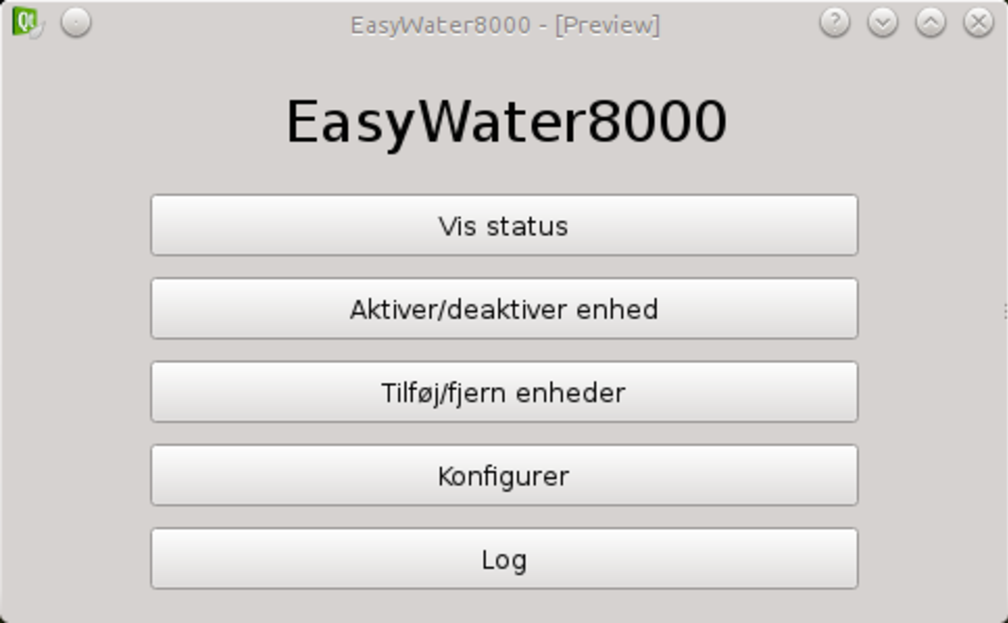
\includegraphics[scale=0.5]{filer/pics/GUI/Start-menu}}
\caption{Skitse af startmenu på GUI}
\label{fig:GUI-Startmenu}
\end{figure}

\subsubsection{Vis Status}
På figur \ref{fig:GUI-aktuel-status} vises den aktuelle status af systemets Enheder. Den øverste række tal er tilkoblede Enheder. Den anden række tal er komponentpakker tilkoblet den enkelte Enhed. Brugeren kan altså bevæge sig rundt og se den seneste udlæsning af data fra de tilkoblede Enheder og deres komponentpakker.

\begin{figure}[htbp] \centering
{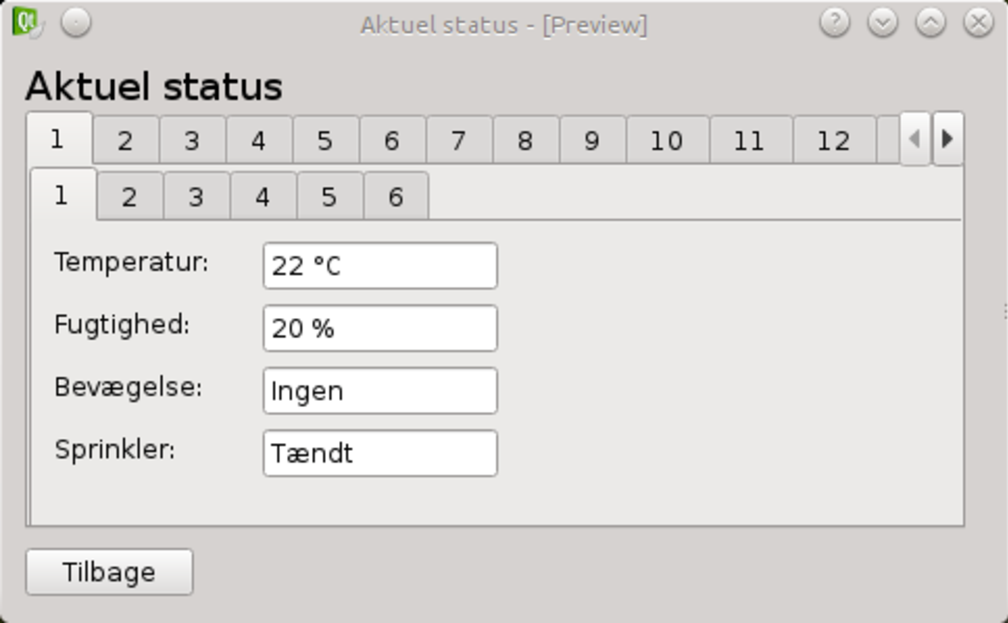
\includegraphics[scale=0.5]{filer/pics/GUI/Aktuel-status}}
\caption{Skitse af ''Vis status'' på GUI}
\label{fig:GUI-aktuel-status}
\end{figure}

\subsubsection{Aktiver og deaktiver enhed}
Skitsen på figur \ref{fig:GUI-aktiver-deaktiver} viser Brugerens mulighed for at aktivere og deaktivere enkelte enheder i systemet. Der præsenteres en liste af opsatte Enheder, hvor man kan markerer den ønskede Enhed og vælge en funktion for denne.

\begin{figure}[htbp] \centering
{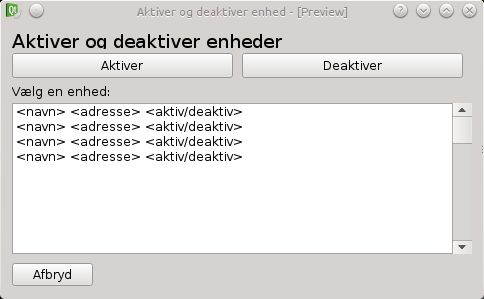
\includegraphics[scale=0.5]{filer/pics/GUI/Aktiver-deaktiver-enheder}}
\caption{Skitse af ''Aktiver og deaktiver enhed'' på GUI}
\label{fig:GUI-aktiver-deaktiver}
\end{figure}

\subsubsection{Tilføj/fjern enheder}
De præsenterede muligheder i forbindelse med at fjerne og tilføje enheder til systemet er vist på figur \ref{fig:GUI-tilfoj-fjern}. Igen vises en liste af opsatte Enheder. Det er muligt at tilføje en ny, eller markerer en eksisterende og fjerne denne.

\begin{figure}[htbp] \centering
{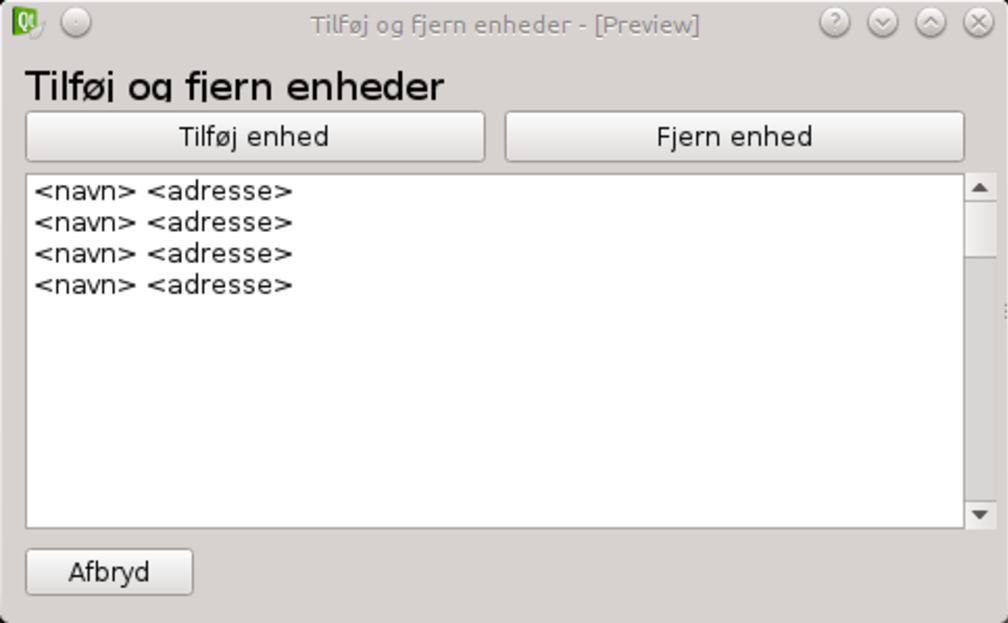
\includegraphics[scale=0.5]{filer/pics/GUI/Tilfoj-fjern-enheder}}
\caption{Skitse af ''Tilføj/fjern enheder'' på GUI}
\label{fig:GUI-tilfoj-fjern}
\end{figure}

\subsubsection{Konfigurer}
Når brugeren skal konfigurere en Enhed, bruges skitsen på figur \ref{fig:GUI-konfigurer}. Her vælger Brugeren hvilken Enhed der skal konfigureres. Vinduet skifter til ''Indstil parametre''-vinduet når en enhed markeres.

\begin{figure}[htbp] \centering
{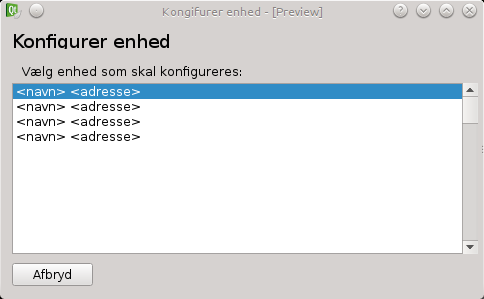
\includegraphics[scale=0.5]{filer/pics/GUI/Konfigurer-enhed}}
\caption{Skitse af ''Konfigurer'' på GUI}
\label{fig:GUI-konfigurer}
\end{figure}

\subsubsection{Indstil parametre}
Når brugeren har valgt en enhed som skal konfigureres vises skærmen på figur \ref{fig:GUI-indstil-parametre}. Her kan brugeren indtaste parametrene for enheden og gemme dem i systemet.

\begin{figure}[htbp] \centering
{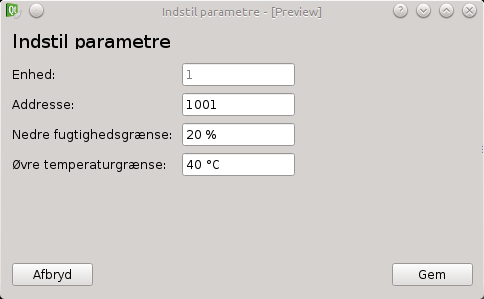
\includegraphics[scale=0.5]{filer/pics/GUI/Indstil-parametre}}
\caption{Skitse af ''Indstil parametre'' på GUI}
\label{fig:GUI-indstil-parametre}
\end{figure}

\subsubsection{Log}
Loggen præsenterer de indsamlede data fra alle Enhederne. Det er muligt at se alle data på en gang, som vist på figur \ref{fig:GUI-log-alle}, hvor den øverste fanerække er numre på opsatte Enheder i systemet, eller man kan vælge de enkelte Enheder og se deres forskellige komponentpakker, som vist på figur \ref{fig:GUI-log-enhed}, hvor den anden fanerække er komponentpakker koblet op på systemet.

\begin{figure}[htbp] \centering
{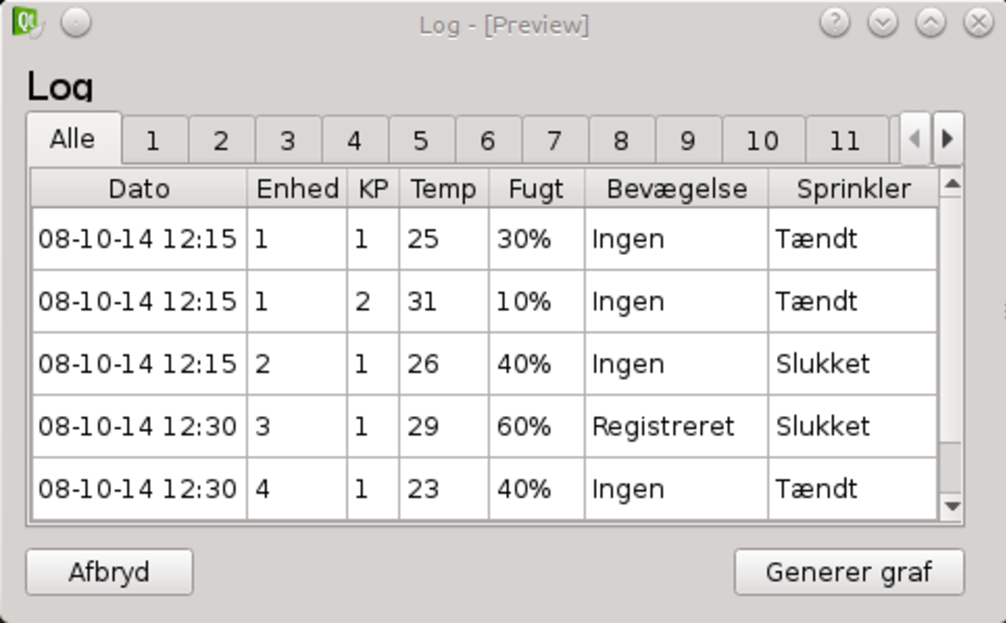
\includegraphics[scale=0.5]{filer/pics/GUI/Log-alle}}
\caption{Skitse af ''Log'' for alle enheder på GUI}
\label{fig:GUI-log-alle}
\end{figure}

\begin{figure}[htbp] \centering
{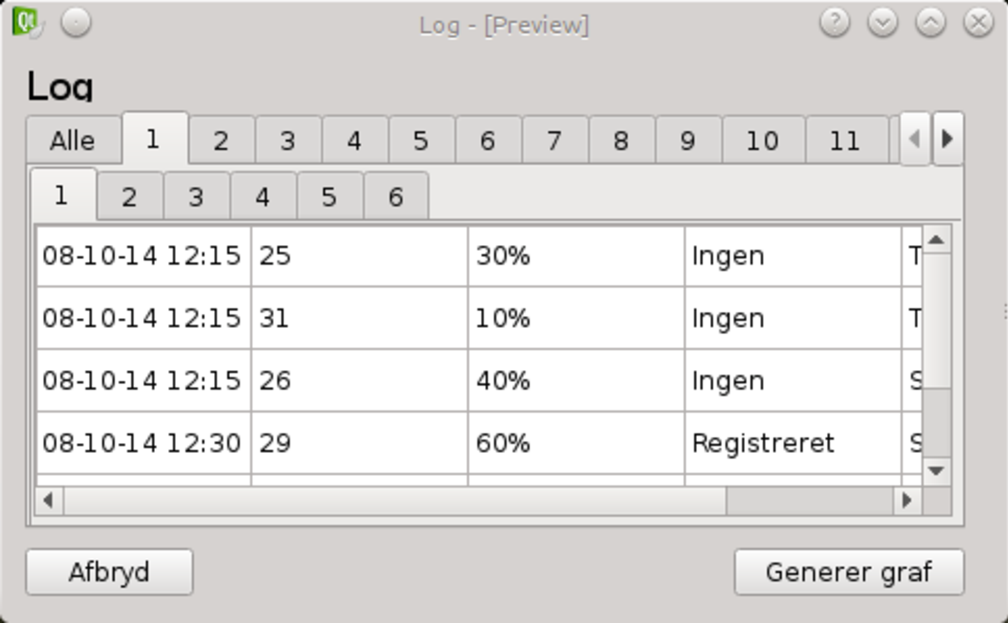
\includegraphics[scale=0.5]{filer/pics/GUI/Log-enhed}}
\caption{Skitse af ''Log'' for enkelt enhed på GUI}
\label{fig:GUI-log-enhed}
\end{figure}



